
Realistically sized programs usually consist
of 100.000s of LOC and hundreds of files.
Instrumenting all of it on the basic block level
could result in an undesirable slowdown,
a large amount of runtime data,
and could even be impossible to instrument
(before instrumentation every file has to be
linked into one intermediate LLVM bytecode file).

To overcome this problem some instrumentation
and analysis strategies can be implemented
using partial instrumentation.

If the speed of the instrumented program is
compromised or the generated datafile is too
large, one can opt to instrument on function
level initially.
This will reduce the size of the datafile
and will result in a fault localization that
is less detailed.
Using these results, however, one can then
select the top ranking files, which are most
likely to contain the fault, for a more
fine-grained instrumentation, for example
on the basic block level.
Less basic blocks are instrumented,
compared to instrumenting the complete program,
resulting in a more manageable datafile and better
performance of the instrumented executable.

	\begin{figure}[h!]
		\begin{center}
		\begin{tabular}{c}
			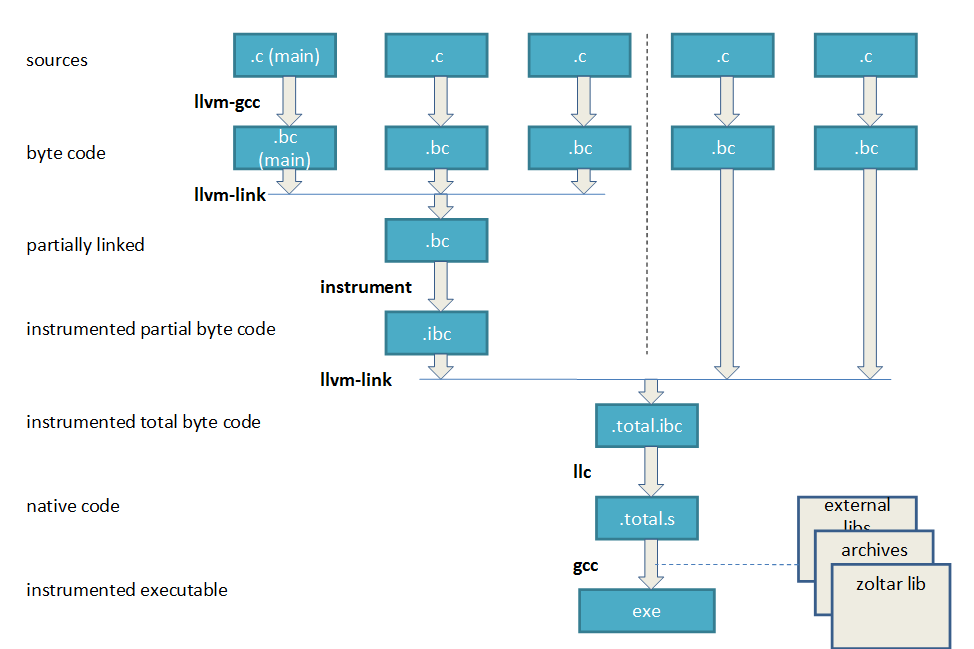
\includegraphics[scale=0.30]{sources/partial_instrumentation.png} \\
		\end{tabular}
		\end{center}
		\caption{Partial instrumentation.}
		\label{fig:partialInstrumentation}
	\end{figure}

The general instrumentation procedure,
supporting partial instrumentation,
is illustrated in Figure \ref{fig:partialInstrumentation}.
It shows that all source files are first
converted to LLVM bytecode.
A selection of these bytecode files,
including the file with the main function,
are then linked together and instrumented.
In the next step, the resulting instrumented bytecode
is linked with the remaining bytecode
that was not instrumented.
Finally, native code is generated and all is
linked with other archives of the program,
external libraries and the Zoltar library.
Note that having internal libraries or archives
can reduce the total size of the linked bytecode
file just before converting to native code.
LLVM could have problems if this were too large.
However, if some of these libraries are to be
instrumented as well, their source files should
be linked to the main source file before instrumenting,
as instrumentation of a program can not be done
on various source files separately.


